%\thispagestyle{plain}

%\section{Foreword}

%I was introduced to role-playing through video games.  Early PC titles like Ultima, Wizardry, and Might \& Magic brought me into fantastical worlds where monsters lurked in every wire frame dungeon waiting to kill your faceless avatars who sought fantastic, randomly generated treasure.  I made my own maps, poorly scribbled on graph paper, complete with locations of traps, merchants, and ambushes.  I named my characters after friends and family -- their victories and failures felt like my own.  With every death or secret trove discovered, I felt like I had accomplished something.  No play session, whether five minutes or five hours, went without its pleasant (or not) surprises.

%Unwittingly I was being prepared for a richer and more in depth experience that transcended the digital world.  I remember checking out the 2\textsuperscript{nd} Edition Advanced rules at my local library.  I knew a little about the license from video games but nothing could prepare me for the wealth of opportunities within those books.  

%Cracking open the original 1989 player's guide, the first illustration you're drawn to is a full-page oil painting by Larry Elmore.  Entitled ``Dragon slayers, and proud of it!" the painting depicts five adventurers triumphantly posing before the body of a very young green dragon dangling from a tree as a fisherman would present his prized catch.  A small wooden box at their feet held gold coins, a few glittering gems poking out here and there.  The adventurers weren't wearing ridiculously exaggerated armor, bikini-mail with bare midriffs and massive cleavage, or wielding fifty-foot long paper-thin swords.  Our heroes were a lightly armored elf archer, a cleric with a hammer and a holy symbol etched on his belt buckle, a massive bearded warrior with rusty chain mail, a smaller raven haired female warrior, and a mysterious looking magic user cloaked in red.

%To me, this picture is how I imagine the quintessential adventurers.  These allies had braved some distant lair, defeated a mighty monster (as even newborn dragons are not to be trifled with), collected a modest treasure, and escaped with treasure (and a few scars) that tell entire stories.  These heroes were the invisible men and women I created in my fantasy video games.  I knew that I held in my hand a gateway into majestic worlds yet to be told and I quickly met many people whose vision we all shared.  These dragon slayers have made a hobbyist out of me and I'm proud of it.

%\vspace{1em}

%\noindent Justen Brown

%\newpage

%\thispagestyle{plain}
 
%\section{Editor's Foreword}

%``Wow!"  That's the sound that I make every time I think about the last year and a half that I labored on this massive compendium of rules and suggestions.  Since February of 2010, \underline{For Gold \& Glory} has consumed most of my spare time.  Though I have done smaller projects in recent years, I haven't been this consumed by a game system since I published my own OGL inspired \underline{Mutazoids3e} back in 2003.  While that project used the (then) new open gaming system and a post apocalyptic setting, as you know by now, \underline{FG\&G} uses the open gaming license to simulate old school rules in a straight fantasy setting.  I felt as if I had come home to a much more familiar territory. 

%Even though I didn't know it at the time, my first gaming experiences were in hybrid games.  Thirty years later, I can now see how my first GM had intricately woven rules from the (then) new, ``Advanced" version of the game with his favorite house rules pulled from the ``Basic" games that came before it and the now infamous RPG magazines of the day: the Dragon, Dungeon, Polyhedron, etc.

%\underline{For Gold \& Glory} pays homage to this hybrid style of gaming.  My primary concern when I took over as editor of \underline{FG\&G} was to lay nothing less than a solid, old school foundation similar in style to the second ``Advanced" version of the game.  My next concern then became to fix any obvious errors and fill in any obviously missing rules.  Whenever possible, the most official sources (such as erratum, official second edition handbooks, ``\textit{Dispel Illusion}", and www.d20srd.org) were consulted.  Next, either the first ``Advanced" version or even one of the ``Basic" versions was consulted.  If no official source could be found, unofficial sources, such as ``\textit{Sage Advice}" was checked, and finally if no source of information could be found, I would consult the forums at www.dragonsfoot.com and attempt to form a consensus.  Justen and I dropped sections of his original manuscript, other sections previously considered optional were added, and all sections were completely reworked.  I attempted to leave stubs in place for many of the optional rules that have not yet been devised.  While my stepson Warren and others found several issues in the core, Adam was of utmost assistance when working with the spells.  He devoured them, and researched dozens of issues I never would have considered.  Lessons learned while working on spells paid off while working on magical items.  Dan came on to the project at this time, checked over the magical items, corrected my punctuation over the entire document, and forced me to be more careful with my run-on sentences.  

%This book is the result.  Despite its size, I certainly don't think it's perfect or complete.  I also don't think everyone will agree with every decision that Justen or I made.  Even so, I am rather pleased with it, not because it represents the way you or I actually play the game, but because it lays a solid foundation for either of us to turn it into the game we will love to play.

%\vspace{1em}

%\hfill Moses Wildermuth

%\hfill July 12, 2012

%\vspace{1em}

%\noindent PS---Always remember that magic is not an exact science but any sufficiently advanced science is indistinguishable from magic, and never forget that it's only a game- HawkWolf

%\newpage

\chapter{}

\begin{multicols}{2}
 
\section{INTRODUCTION TO THE GAME}

In the early 1970s, a number of wargamers began to modify and elaborate on the rules of the miniatures games that they were playing. Among these people were Dave Arneson and Gary Gygax, and between them, they developed the first roleplaying game. Whereas previous games focused on armies, their game focused on individual characters. This individual focus, and the recurring characters and settings that it implied, led to the creation of the roleplaying concept. Together, Arneson and Gygax published the resulting game in 1974.

The original roleplaying game was soon expanded upon with a number of supplemental rules. Drawing upon these, Gygax created the ``advanced" version of the game as a reference for tournament play and as a seperate game in which Arneson's influence was legally diminished. This ``advanced" game was a huge success, spawning hundreds of tie-in products. In the late 1980s, a second edition of the ``advanced" game was developed by David Cook, Steve Winter, and Jon Pickens in order to streamline and clarify the presentation of the rules, as well as to consolidate into the core game some of the new rules published since the debut of the first edition of the ``advanced" game.

The second edition of the ``advanced" game was retired in 2000 and went out of print, but this book seeks to recover from that loss. \textit{For Gold \& Glory}\texttrademark{} uses the Open Gaming License to emulate the rules of that game, free for use in play and as a basis to publish additional material upon, under the terms of the OGL. As it is free to distribute and copy, it can never go out of print. 

%In 1974, E. Gary Gygax and Dave Arneson created the rules to the world's first published Role Playing Game.  Combining improvisational character acting with modified war-gaming rules to support single players, ``The Fantasy Medieval War game" became a major success among tabletop gamers and young adults alike.  Gygax continued to expand on his original concept and in 1977 he released the first edition ``Advanced" rules based on the original TFMW.  

%Gygax billed his new rules as ``neither an expansion nor a revision of the old game, it is a new game".  For ten years the Advanced product line remained strong, seeing many published adventures, a monthly magazine, and supplemental material that expanded the rules.  Having left the company, TSR built upon Gygax's Advanced line to create a ``2\textsuperscript{nd} Edition" in 1989 designed by David ``Zeb" Cook and developed by Steve Winter and Jon Pickens.  

%For Gold \& Glory is an Open Game License interpretation of Zeb Cook's 2\textsuperscript{nd} Edition rules.  All material contained within is free for use, distribution, copying, and updating within the confines of the OGL.  The rules remain mostly intact but the descriptions have changed for the sake of brevity, clarity, and ease of reference. For Gold \& Glory gives role players a complete reference to 2\textsuperscript{nd} Edition ``core material" and allows publishers to release original or new material using 2\textsuperscript{nd} Edition rules.

\subsection{WHAT IS A ROLE-PLAYING GAME?}
A role playing game combines the rules aspects of a board game with the free form acting found in traditional role-play.  Players assume the role of intrepid heroes (or dastardly villains) and their interactions with the world they live in.  Players act as their avatars would with a fictional background and personality.  

What separates role-playing from all other games is the variable nature.  Heroes win and lose as the result of good planning, experience, and sharp skills or lack thereof.  However, just like real life, circumstances can get the better of you as events can sway in either direction at the drop of a hat (or dice, in the game's case).  

The players shape the world and the Game Master creates the world.  The rules remain the same, but unlike most games the playing field constantly changes.  Role-playing is unique because every choice has a reaction.  Sometimes it's blatant but often subtle.  You can play the game for years and never recreate the same experience twice.  

 
\subsection{THE GOLDEN RULE}
Have fun.  Role-playing is a shared experience that relies on the teamwork of everyone at the table.  If people aren't having fun then the problem needs to be identified quickly, whether it's a problem player or noticeable distraction.  If a single person is ruining the enjoyment for everyone else, they should be politely notified of their behavior and the situation corrected without detracting from the game.  Arguments naturally devolve from interpretations of the rules but regardless of any situation the GM has the final say in all matters.  The only important thing at the table is the game and the enjoyment of everyone.

\subsection{A WORD ON METAGAMING}
Metagaming is a term referring to a character that has knowledge that only the player could obtain.  This is usually knowledge regarding monsters, spells, or item functions.  The challenge of role-playing is feigning ignorance.  Players are discouraged from acting upon knowledge their characters wouldn't have.  Remember that \textit{FG\&G}\texttrademark{} is a game of high fantasy and magic where literally anything is possible from exploring the stars to time travel.  This is a game where gods can walk the earth\ldots or not.  The GM is ``God" but should be impartial in his rulings.

\subsection{REQUIRED MATERIALS}
To play this game you need a player willing to be the Game Master (GM) and at least one player to run a character.  The Game Master creates and runs the world while the players create characters to experience the world.  Four to five characters are optimal---the more players, the slower the game plays.  In addition to a copy of this rule set you'll also need some paper, graphing paper for maps although combat relies very little on exact placement, some miniatures or character markers if you prefer, pencils, and a set of funny dice (d4, d6, d8, d10, d12, and d20).  

\subsection{CORE MECHANIC}
The basis on which the game runs is ``If it's not covered by the rules, roll d20 and add or subtract modifiers."  There are numerous situations that cannot be covered in a single document.  In cases where an action seems probable, a player is encouraged to roll a d20; high numbers favor their character.  Positive modifiers can be applied for easy situations such as masterwork tools and negative modifiers can be applied for difficult situations such as poor visibility.  As a rule of thumb, situational modifiers should be applied in even numbers such as $-2$ ($-10$\%) or +4 (+20\%).  The higher the bonus means the easier the task and vice versa for penalties.

 
\subsection{A NOTE ABOUT PRONOUNS}
The male pronoun (he, him, his) is used regularly throughout this document for ease of use.  It does not reflect gender exclusivity.

\section{AN EXAMPLE OF PLAY}
This example is to ease new players into how a typical game of \textit{For Gold \& Glory}\texttrademark{} is played.  A fighter, ranger, thief, and wizard (the four players) have been tasked by a nearby village to clear out the evil infesting a nearby moat house.  The PCs easily dispatched the giant frogs that ambushed them in the marshes and are now approaching the ruined drawbridge.

\paragraph{GM:} Wiping the frog blood from your weapons, you approach a drawbridge.  Half of it has been battered through and the holes patched with wooden planks, the wood having long rotten.  The chains have fallen and are completely rusted.

\paragraph{Wizard:} I'm not setting foot on that!

\paragraph{Thief:} Let me prod it with my 10' pole!

\paragraph{Fighter:} Forget it.  I'm the heaviest.  Attach this rope around my waist, hand it to Ranger, and walk across testing each plank.

\paragraph{Ranger:} A sound plan.

\paragraph{GM:} The wood has rotted but it holds up easily under your weight.  The rest of the party crosses with no problems.  Before you are massive wooden doors serving as gates -- one hanging open on a great hinge and the other is splintered and shored closed from the inside.  Boot prints are visible leading out from the gates.

\paragraph{Thief:} Where there are tracks, there's bound to be treasure.

\paragraph{Ranger:} Or, more accurately, trouble.  Fighter, cover me.  Stooping low, I follow the tracks in.  What do I see?

\paragraph{GM:} (Secretly rolls dice.  He determines that two brigands keeping watch spot the party and stealthily run off to warn their leader.) The tracks lead into a ruined courtyard.  Great stone steps lead up to the moat house's main keep, the large oak doors rotten and ajar.  The remains of a watchtower looms behind you, its wooden doors closed.

\paragraph{Ranger:} About how many tracks are there? (Ranger rolls a skill check for his tracking ability)

\paragraph{GM:} Six or seven distinct tracks.  It's hard to tell because the tracks slide about on the wet surface.  Two tracks are fresh, though, only a minute or two old.

\paragraph{Ranger:} Weapons out, everyone. Proceed in formation to the keep.

\paragraph{Wizard:} I don't like being out in the open.  I cast shield on myself.  What do we hear?

\paragraph{GM:} Aside from your own chanting, strange sounds from inside the keep echo out and reverberate along the walls.

\paragraph{Thief:} Hmm, that watchtower shouldn't go unchecked.  I peek inside.

\paragraph{Ranger:} Hey! Stay in formation!

\paragraph{GM:} Creeping over to the doors, you push them open.  A few bones are scattered among the dirt but the gleam of many coins catches your eye.

\paragraph{Thief:} Jackpot!  I rush in and scoop up some coins.

\paragraph{Fighter:} Stop you idiot!
 
\paragraph{GM:} Thief runs in with his coin purse open ready to snatch up some gold.  There's a hissing sound and a rush of air as a huge spider, the size of a bull mastiff, drops down.  (Rolls d6 to see if Thief is surprised on a 1-5 -- GM rolls a 6 meaning Thief isn't surprised.) Your keen senses are enough to keep you alert but the spider presses in to attack.

\paragraph{Thief:} Help me!

\paragraph{Wizard:} Argh!  I hate spiders!!

\paragraph{Fighter:} Attack!

\paragraph{GM:} Hold it, I'm not done yet.  As the spider drops down you guys immediately hear multiple footsteps echo out the keep.  Eight rough and tumble men wearing studded leather armor and wielding flails come rushing out followed by a larger, meaner looking man wearing chain armor, a shield, and wielding a long sword.  He speaks ``More adventurers?!  Your heads will line my trophy wall, Haha!"

\paragraph{Ranger:} I'll see to it this land is cleansed of your evil, brigand!  Charge!!

\subparagraph{} The game continues as the PCs fight out this encounter.  Thief is in a bad spot, fighting a huge spider alone, but he could gain the advantage by striking first.  The other three PCs must contend with triple their numbers but Fighter and Ranger can hold their own in melee, the brigands are poorly equipped, and Wizard can cast sleep which may be the key to winning the battle.  

The events could've been different depending on the party's actions.  The two brigands standing watch could've been surprised and likely would have run off screaming or surrendered.  The PCs could've investigated the watchtower first, fighting the spider alone and likely making quick work of it.  The brigand leader, a coward at heart, could've ordered a retreat while taking with all their treasure with them but instead he pressed on after seeing the party was only three strong (he can't see Thief who is in the watchtower).  

Every game is different and the party's actions shape the world around them.  This is the key to good roleplaying.
 
\section{GLOSSARY}

\paragraph{Ability:} \index{Ability Scores}One of six attributes that determine the basic strong points and weak points of a character.  These attributes are strength, dexterity, constitution, intelligence, wisdom, and charisma.  

\paragraph{Ability Check:} \index{Ability Check}A roll of 1d20, plus modifiers, against a relevant ability score.  If the result is equal to or less than your character's ability score the action succeeds.  As a general rule, any action not covered by the rules should be handled with an ability check.  For example, use a dexterity check to swing off a chandelier or an intelligence check to navigate a difficult maze.  The GM may apply penalties based on the situation such as $-8$ for a fighter trying to pick a lock ($-2$ for not having tools and $-6$ for not being a trained thief).   If an action takes longer than a few seconds, assume a person can perform that action on a successful check for one round (one minute) before having to re-roll.

\paragraph{Alignment:} \index{Alignment}Reflects the characters attitude and personality.  Alignment is a guideline, not an all-encompassing rule.  A good character may lie to protect an innocent ally, while an evil person's lie is likely to be entirely self-serving and harmful.

\paragraph{Armor Class (``AC"):} \index{Armor Class}The defensive rating of a character, or how difficult they are to hit.  AC begins at base 10 (unarmored, no modifiers) and caps at $-10$ (highest armor value regardless of modifiers).  Penalties increase AC and bonuses reduce it.  AC is an abstraction; failing to hit an opponent's AC doesn't necessarily mean a ‘miss' but rather the weapon scraped across armor harmlessly, or the blow was deflected.

\paragraph{Attack Roll:} \index{Attack Roll}1d20 plus modifiers.  Any bonus ``to hit" is added to the attack roll.  The attack roll is cross-referenced with THACO to determine a successful hit.

\paragraph{Common:} The generic, universal language that all player characters know how to speak, read, and write.  Often, all civilized races and societies that interact with one another share this language.  

\paragraph{Creature:} A collective term for PCs and NPCs.  Sometimes used interchangeably with ``character" or ``monster".

\paragraph{d\#:}  Abbreviation for die or dice.  By itself, it means a single die while a number preceding indicates the number of die or dice to roll (E.G. 3d6 means roll three sets of six dice).

\paragraph{d3:}  Roll 1d6; a result of 1-2 is considered a 1, 3-4 is considered a 2, and 5-6 is considered a 3.

\paragraph{d100 or d\%:}  Either an actual 100 sided dice or roll 2d10 and denote which is the 10s die and which is the 1s die.  A roll of 10 on either die is considered a 0.  Rolling two 0s is equal to 100.

\index{Damage}\paragraph{Damage:} The effect of a successful attack subtracted from a creature's hit points.

\index{Demi-human}\paragraph{Demi-human:} Any non-human player character race.  

\paragraph{Dual-class Character:} \index{Dual-class Characters}A human who stops advancing in their current class to advance in another. Demi-humans cannot dual class.

\paragraph{Effective Area:} The area in which a device, creature or character's power works.  Unless stated otherwise, all creatures caught in the area are subject to the effects, regardless of disposition.

\paragraph{Energy drain:} \index{Energy Drain}A special power that allows a creature to drain the life energy in the form of class levels from a character.

\paragraph{Experience points (``XP"):} \index{Experience}Points characters earn from the GM.  When XP reaches a certain level, their character advances learning new abilities and becoming more powerful.

\paragraph{Game Master (``GM"):} The player who controls the flow of the game, creates encounters, and adjudicates the rules.

\paragraph{Henchman:} \index{Henchmen}Non-player character that is loyal to a specific PC.  The PC in question usually controls the henchman's actions but is expected to treat the henchman fairly. In cases of abuse, a henchman should be role-played by the GM.  The total number of henchmen a PC can ever have is based on the PC's charisma score.

\paragraph{Hireling:} \index{Hirelings}Non-player characters hired for a particular task and that usually stay under control of the GM.  Hirelings are loyal, so long as the pay is good, and the job in question isn't against their nature.

\index{Hit Dice}\paragraph{Hit dice:} Dice rolled to determine a character's hit points.  After a certain level, hit dice are no longer obtained.  Hit point modifiers gained from constitution are only added to hit dice, never levels.

\index{Hit Points}\paragraph{Hit points (``HP"):} A number representing the overall health of a character.  Hit points are an abstraction; higher-level characters are capable of shrugging off blows that would have killed weaker characters.  An attack that deals 1 HP against a creature with 2 HP is a vicious blow but the same attack against a creature with 20 HP is hardly a scratch.  

\paragraph{Infravision:} \index{Infravision}The ability to see in non-magical darkness.  Infravision is black and white only; color must be discerned in natural light.

\paragraph{Initiative:} \index{Initiative}A 1d10 roll made by opposing parties in combat.  Lower initiatives go before higher initiatives.  All actions a party makes happen simultaneously before proceeding to the next party in the initiative order.

\paragraph{Level:} Generally used as a measure of power for characters, dungeons, or spells.  The higher the level, the stronger the aspect is.

\paragraph{Melee:} Combat made through direct contact, either through natural or manufactured weapons.

\paragraph{Missile combat:} Attacking using a ranged weapon, either powered by a weapon or thrown.

\paragraph{Movement Value/Speed (``MV"):} \index{Speed}A number representing the distance a character can cover in a single round.  Movement value (or sometimes referred to as ‘speed') is represented in miles, yards, or feet depending on whether the characters are traveling overland, exploring open terrain, navigating enclosed areas, or fighting.

\paragraph{Multi-class character:} \index{Multi-class Characters}A demi-human with more than one class.  Humans cannot multi-class.

\paragraph{Non-player Character (``NPC"):} All characters controlled by the GM.

\paragraph{Object:} Any inanimate, unintelligent item, organic or not.  Some objects are magically intelligent and can be treated as creatures.

\index{Races}\paragraph{Race:} A player character's species. These include human, elf, half-elf, dwarf, halfling, and gnome.

\paragraph{Rate of fire (``ROF"):} The number of times a ranged weapon can be used to attack, represented as (\# of attacks)/(per round).  An ROF of 3/1 means three attacks per round.  An ROF of 1/2 means one attack every other round.

\paragraph{Round:} Measurement of in-game time equal to 1 minute.  In combat, characters can generally perform one action.  Rounds are an abstraction and in combat encompass more than simple attacking and moving.  Attackers feint, dodge blows, and move into favorable positions.

\paragraph{Saving Throw:} \index{Saving Throws}A character's ability to resist the effects of special attacks such as magic, poison, or a dragon's breath.  Success is determined by rolling 1d20 and meeting or beating the character's modified save.  Penalties increase saving throws, while bonuses decrease it.
 
\paragraph{Size Category:} \index{Size}All creatures have a size category that can affect the type of equipment they need, the amount of damage done to them and the types of spells cast against them.  Most humanoids are man-sized, thus equipment is sized for them.

\noindent
%\rowcolors{2}{gray}{white}
\begin{tabular}{|p{.45\columnwidth}|p{.45\columnwidth}|}
\hline
Size	& Examples \\
\hline\hline
\rowcolor[gray]{.9}Tiny-sized or smaller 	& Pixie, frog \\
Small-sized	& Halfling, large spider \\
\rowcolor[gray]{.9}Man-sized	& Human, riding dog \\
Large-sized 	& Ogre, bear \\
\rowcolor[gray]{.9}Huge-sized	& Giant, behir \\
Gigantic-sized	& Titan, tarrasque \\
\hline
\end{tabular}

\paragraph{Surprise:} \index{Surprise}The chance a party may be surprised before an encounter.  When two or more parties may be surprised, the GM rolls a surprise check of 1d10.  On a 1-3, that character or group is surprised.  It's possible for all parties to be surprised at the same time.

\paragraph{To Hit A Combat Opponent (``THACO"):} \index{THACO}This number represents a character's ability to successfully hit a target.  Subtract the defender's AC from the attacker's THACO -- the attack roll must equal or exceed this modified number in order to successfully hit.  Remember that double negatives (subtracting a negative from a positive) add to the number, making it more difficult to hit.  

Bonuses to hit decrease THACO and penalties increase it.  Under no circumstances can THACO be reduced below 1.  If a bonus would reduce it below 1, discard the remainder.

\paragraph{Turn:} Measurement of in-game time equal to 10 minutes.

\paragraph{Turn Undead:} \index{Turn Undead}The magical ability to channel divine power to turn away or destroy undead.
 
\section{CHARACTER GENERATION BASICS}

To create a character to play in \textit{For Gold \& Glory}\texttrademark{}, read through Chapters 1-6.  These cover all aspects of the player character.  If there's a term you don't understand, check the glossary or keep reading.  Some terms are explained in more detail during later chapters.

You'll keep your character recorded on a sheet of paper.  Some people prefer fancy, pre-made character sheets but a simple index card or lined notebook paper will do.

\subsubsection*{Chapter 1: Roll Ability Scores}
Your character's six ability scores are his ``backbone" and determine his strong points and weak points.

\subsubsection*{Chapter 2: Choose Race}
Each race has its own advantages and disadvantages, special abilities, and movement value.

\subsubsection*{Chapter 3: Choose Class}
Your character's class is like his job.  Class determines combat skills (THACO), health (hit points), endurance (saving throws), and special abilities like stealth or magic.

\subsubsection*{Chapter 4: Choose Alignment}
Your character's alignment is his moral compass, or complete lack thereof, that influences his personality and choices.  Alignment isn't a straight jacket that limits role-play but rather a tool to help guide the decisions you make for your character.  

\subsubsection*{Chapter 5 \& 6: Choose Skills}
This is where your character's previous life experience and training shape a future hero, and you determine his favored or signature weapon(s) and other attack methods that he employs in battle.  If your character is a single class fighter, he will now gain his greatest advantages over the other classes, with the most number of options and interesting combinations.  This is due to a single class fighter's uniquely singular focus on combat.

\subsubsection*{Chapter 7: Purchase Equipment}
With your character finished, it's time to outfit him.  His starting gear could spell the difference between life and death, so choose affordable equipment that will help your character survive long enough to collect more treasure and find better gear.

\noindent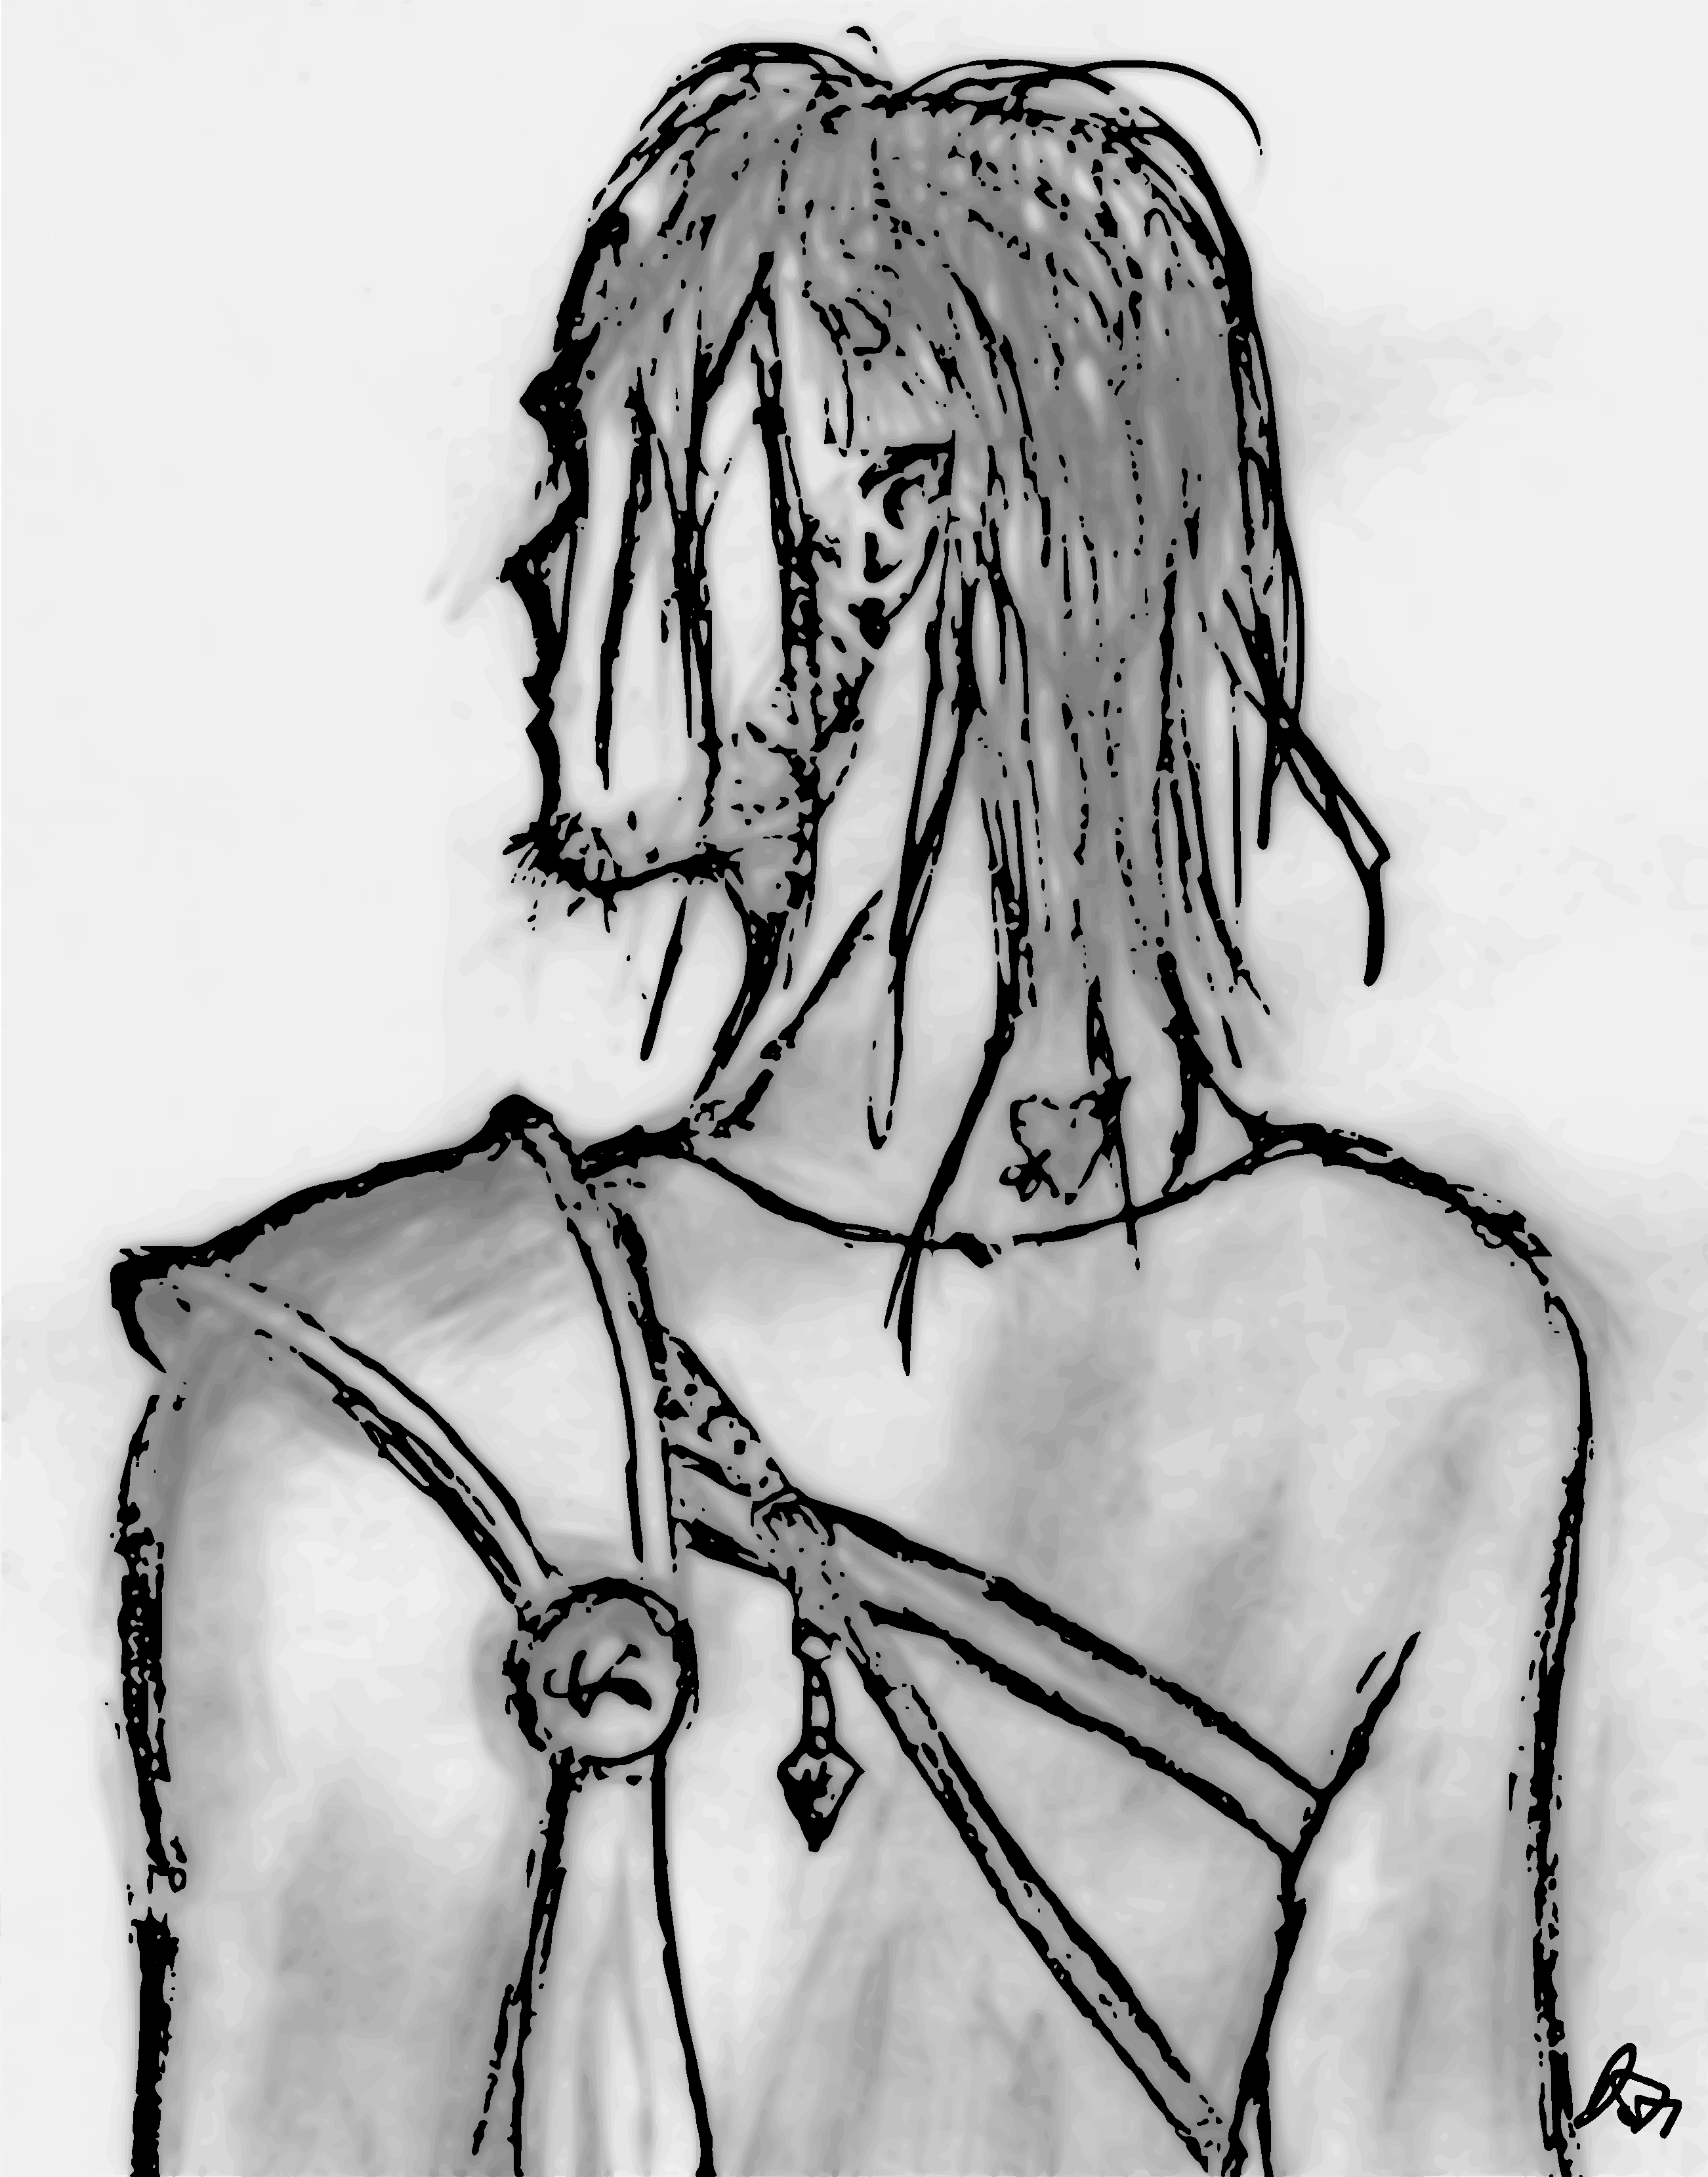
\includegraphics[width=\columnwidth]{drothanthenovice.pdf}\label{drothanthenovice}


\end{multicols}
